\documentclass[journal,12pt,twocolumn]{IEEEtran}
%
\usepackage{setspace}
\usepackage{gensymb}
%\doublespacing
\singlespacing

%\usepackage{graphicx}
%\usepackage{amssymb}
%\usepackage{relsize}
\usepackage[cmex10]{amsmath}
%\usepackage{amsthm}
%\interdisplaylinepenalty=2500
%\savesymbol{iint}
%\usepackage{txfonts}
%\restoresymbol{TXF}{iint}
%\usepackage{wasysym}
\usepackage{amsthm}
%\usepackage{iithtlc}
\usepackage{mathrsfs}
\usepackage{txfonts}
\usepackage{stfloats}
\usepackage{bm}
\usepackage{cite}
\usepackage{cases}
\usepackage{subfig}
%\usepackage{xtab}
\usepackage{longtable}
\usepackage{multirow}
%\usepackage{algorithm}
%\usepackage{algpseudocode}
\usepackage{enumitem}
\usepackage{mathtools}
\usepackage{steinmetz}
\usepackage{tikz}
\usepackage{circuitikz}
\usepackage{verbatim}
\usepackage{tfrupee}
\usepackage[breaklinks=true]{hyperref}
%\usepackage{stmaryrd}
\usepackage{tkz-euclide} % loads  TikZ and tkz-base
%\usetkzobj{all}
\usetikzlibrary{calc,math}
\usepackage{listings}
    \usepackage{color}                                            %%
    \usepackage{array}                                            %%
    \usepackage{longtable}                                        %%
    \usepackage{calc}                                             %%
    \usepackage{multirow}                                         %%
    \usepackage{hhline}                                           %%
    \usepackage{ifthen}                                           %%
  %optionally (for landscape tables embedded in another document): %%
    \usepackage{lscape}     
\usepackage{multicol}
\usepackage{chngcntr}
%\usepackage{enumerate}

%\usepackage{wasysym}
%\newcounter{MYtempeqncnt}
\DeclareMathOperator*{\Res}{Res}
%\renewcommand{\baselinestretch}{2}
\renewcommand\thesection{\arabic{section}}
\renewcommand\thesubsection{\thesection.\arabic{subsection}}
\renewcommand\thesubsubsection{\thesubsection.\arabic{subsubsection}}

\renewcommand\thesectiondis{\arabic{section}}
\renewcommand\thesubsectiondis{\thesectiondis.\arabic{subsection}}
\renewcommand\thesubsubsectiondis{\thesubsectiondis.\arabic{subsubsection}}

% correct bad hyphenation here
\hyphenation{op-tical net-works semi-conduc-tor}
\def\inputGnumericTable{}                                 %%

\lstset{
%language=C,
frame=single, 
breaklines=true,
columns=fullflexible
}
%\lstset{
%language=tex,
%frame=single, 
%breaklines=true
%}

\begin{document}
%


\newtheorem{theorem}{Theorem}[section]
\newtheorem{problem}{Problem}
\newtheorem{proposition}{Proposition}[section]
\newtheorem{lemma}{Lemma}[section]
\newtheorem{corollary}[theorem]{Corollary}
\newtheorem{example}{Example}[section]
\newtheorem{definition}[problem]{Definition}
%\newtheorem{thm}{Theorem}[section] 
%\newtheorem{defn}[thm]{Definition}
%\newtheorem{algorithm}{Algorithm}[section]
%\newtheorem{cor}{Corollary}
\newcommand{\BEQA}{\begin{eqnarray}}
\newcommand{\EEQA}{\end{eqnarray}}
\newcommand{\define}{\stackrel{\triangle}{=}}

\bibliographystyle{IEEEtran}
%\bibliographystyle{ieeetr}


\providecommand{\mbf}{\mathbf}
\providecommand{\pr}[1]{\ensuremath{\Pr\left(#1\right)}}
\providecommand{\qfunc}[1]{\ensuremath{Q\left(#1\right)}}
\providecommand{\sbrak}[1]{\ensuremath{{}\left[#1\right]}}
\providecommand{\lsbrak}[1]{\ensuremath{{}\left[#1\right.}}
\providecommand{\rsbrak}[1]{\ensuremath{{}\left.#1\right]}}
\providecommand{\brak}[1]{\ensuremath{\left(#1\right)}}
\providecommand{\lbrak}[1]{\ensuremath{\left(#1\right.}}
\providecommand{\rbrak}[1]{\ensuremath{\left.#1\right)}}
\providecommand{\cbrak}[1]{\ensuremath{\left\{#1\right\}}}
\providecommand{\lcbrak}[1]{\ensuremath{\left\{#1\right.}}
\providecommand{\rcbrak}[1]{\ensuremath{\left.#1\right\}}}
\theoremstyle{remark}
\newtheorem{rem}{Remark}
\newcommand{\sgn}{\mathop{\mathrm{sgn}}}
\providecommand{\abs}[1]{\left\vert#1\right\vert}
\providecommand{\res}[1]{\Res\displaylimits_{#1}} 
\providecommand{\norm}[1]{\left\lVert#1\right\rVert}
%\providecommand{\norm}[1]{\lVert#1\rVert}
\providecommand{\mtx}[1]{\mathbf{#1}}
\providecommand{\mean}[1]{E\left[ #1 \right]}
\providecommand{\fourier}{\overset{\mathcal{F}}{ \rightleftharpoons}}
%\providecommand{\hilbert}{\overset{\mathcal{H}}{ \rightleftharpoons}}
\providecommand{\system}{\overset{\mathcal{H}}{ \longleftrightarrow}}
	%\newcommand{\solution}[2]{\textbf{Solution:}{#1}}
\newcommand{\solution}{\noindent \textbf{Solution: }}
\newcommand{\cosec}{\,\text{cosec}\,}
\providecommand{\dec}[2]{\ensuremath{\overset{#1}{\underset{#2}{\gtrless}}}}
\newcommand{\myvec}[1]{\ensuremath{\begin{pmatrix}#1\end{pmatrix}}}
\newcommand{\mydet}[1]{\ensuremath{\begin{vmatrix}#1\end{vmatrix}}}
%\numberwithin{equation}{section}
\numberwithin{equation}{subsection}
%\numberwithin{problem}{section}
%\numberwithin{definition}{section}
\makeatletter
\@addtoreset{figure}{problem}
\makeatother

\let\StandardTheFigure\thefigure
\let\vec\mathbf
%\renewcommand{\thefigure}{\theproblem.\arabic{figure}}
\renewcommand{\thefigure}{\theproblem}
%\setlist[enumerate,1]{before=\renewcommand\theequation{\theenumi.\arabic{equation}}
%\counterwithin{equation}{enumi}


%\renewcommand{\theequation}{\arabic{subsection}.\arabic{equation}}

\def\putbox#1#2#3{\makebox[0in][l]{\makebox[#1][l]{}\raisebox{\baselineskip}[0in][0in]{\raisebox{#2}[0in][0in]{#3}}}}
     \def\rightbox#1{\makebox[0in][r]{#1}}
     \def\centbox#1{\makebox[0in]{#1}}
     \def\topbox#1{\raisebox{-\baselineskip}[0in][0in]{#1}}
     \def\midbox#1{\raisebox{-0.5\baselineskip}[0in][0in]{#1}}

\vspace{3cm}


\title{Problem: 11.11.3.9}
\author{Nikam Pratik Balasaheb (EE21BTECH11037)}





% make the title area
\maketitle

\newpage

%\tableofcontents

\bigskip

\renewcommand{\thefigure}{\theenumi}
\renewcommand{\thetable}{\theenumi}
%\renewcommand{\theequation}{\theenumi}

\section{Problem}
Find the co-ordinates of the foci, the vertices, the length of major axis, the minor axis, the eccentricity and the length of latus rectum of the ellipse $4x^2+9y^2=36$.

\section{Solution}
\begin{enumerate}

	\item Given ellipse equation:
\begin{align}
	\vec{x}^{\top} \vec{V} \vec{x} + 2 \vec{u}^{\top}\vec{x} +f &= 0\\
	here,\;\;
	\vec{V} &= \myvec{\frac{4}{9} & 0\\0&1}\\
	f &= -4\\
	\vec{u} &= \myvec{0\\0}
\end{align}

\item points of intersection of a line $\vec{x} = \vec{A}+ \mu\vec{h}$ with ellipse are given by:
\begin{multline}
	\mu_i = \frac{1}{\vec{m}^{\top}\vec{V}\vec{m}} \brak{-m^{\top}\brak{\vec{V}\vec{h}+\vec{u}} \pm \sqrt{\brak{\vec{m}^{\top}\brak{\vec{V}\vec{h}+\vec{u}}}^2 - \text{g}\brak{\vec{h}}\brak{\vec{m}^{\top}\vec{V}\vec{m}}}}
\end{multline}

where,
\begin{align}
	\text{g}\brak{\vec{h}} = \vec{h}^{\top}\vec{V}\vec{h} + 2\vec{u}^{\top}\vec{h} +f
\end{align}


\item Center of the ellipse,
	\begin{align}
		\vec{C} &= -\vec{V}^{-1}u\\
			&= \myvec{0\\0}
	\end{align}

\item Major axis
	\begin{align}
		\myvec{0&1}\vec{x} &= 0\\
		i.e., \; \vec{x} &= \mu \myvec{1\\0}
	\end{align}
\item Vertices

Vertices lie on major axis, therefore let
\begin{align}
	\vec{v} &= {\mu}_i \myvec{1\\0}\\
	m^{\top}\vec{V}\vec{m} &= \frac{4}{9}\\
	\vec{m}^{top}\brak{\vec{V}\vec{h}+\vec{u}} &= 0\\
	g(h) &= -4\\
	{\mu}_i &= \frac{0 \pm \sqrt{0 - \brak{-4}\frac{4}{9}}}{\frac{4}{9}}\\
		&= \pm 3
\end{align}
Vertices are $\myvec{3\\0}$ and $\myvec{-3\\0}$ 

\item Length of major axis
\begin{align}
	\text{length of major axis}	&= \text{distance between vertices}\\
					&= \norm{ \vec{v_1} - \vec{v_2}}\\
					&=6
\end{align}

\item minor axis
	\begin{align}
	\myvec{1&0} \vec{x} = 0\\
	i.e., \;\; \vec{x} = \mu \myvec{0\\1}\\	
	m^{\top}\vec{V}\vec{m} &= 1\\
	\vec{m}^{\top}\brak{\vec{V}\vec{h}+\vec{u}} &= 0\\
	g(h) &= -4\\
	{\mu}_i &= 0 \pm \sqrt{0 - \brak{-4}}\\
		&= \pm 2
	\end{align}

Points of intersection of minor axis with ellipse be $\mu_i \myvec{0\\1}$

\begin{align}
	\text{Points of intersection of minor axis with ellipse} &= \pm \myvec{0\\2}
\end{align}

\item Length of minor axis
\begin{align}
	\text{length of minor axis} &= \text{distance between Points of intersection}\\
				    &= 4
\end{align}

Normal to directrix,
\begin{align}
	\vec{n} &= \text{direction vector of major axis}\\
		&= \myvec{1\\0} \label
\end{align}
\begin{align}
	\vec{V} &= \norm{\vec{n}}^2 \vec{I} - e^2 \vec{n} \vec{n}^{\top} = \myvec{\frac{4}{9}&0\\0&1}\\	\label{eq:1}
	\vec{u} &= ce^2 \vec{n} - \norm{\vec{n}}^2\vec{F} = \myvec{0\\0}\\	\label{eq:2}
	f &= \norm{\vec{n}}^2 \norm{\vec{F}}^2 - c^2e^2  = -4
\end{align}

\item Eccentricity
\begin{align}
	e = \frac{\sqrt{5}}{3} 
\end{align}

\begin{align}
	\vec{F} = \frac{5c}{9}\myvec{1\\0}
\end{align}

\begin{align}
	c &= \pm \frac{9}{\sqrt{5}}
\end{align}

\item Foci 
\begin{align}
	\vec{F} &= \myvec{ \pm \sqrt{5} \\0}
\end{align}

\item equation of Latus Recta
\begin{align}
	\vec{n}^{\top} \brak{\vec{x} -\vec{F}} &= 0\\
	\myvec{ 1&0} \vec{x} &= 3\\
	i.e., \vec{x} &= \myvec{3\\0} + \mu \myvec{0\\1} 
\end{align}

Let points of intersection of latus rectum and curve be,
\begin{align}
	\vec{x} = \vec{F} + \mu_i \vec{m}
\end{align}


here,
\begin{align}
	m^{\top}\vec{V}\vec{m} &= 1\\
	\vec{m}^{\top}\brak{\vec{V}\vec{h}+\vec{u}} &= 0 \\
	g(h) &= -\frac{16}{9}\\
	{\mu}_i &= {0 \pm \sqrt{0 - \brak{-1}\frac{16}{9}}}\\
		&= \pm \frac{4}{3}
\end{align}

\item Length of latus recta
\begin{align}
\text{length of latus recta} &= \text{distance between points of intersection}\\
&= \frac{8}{3}
\end{align}

\end{enumerate}

\begin{table}[h!]
\begin{center}
%%%%%%%%%%%%%%%%%%%%%%%%%%%%%%%%%%%%%%%%%%%%%%%%%%%%%%%%%%%%%%%%%%%%%%
%%                                                                  %%
%%  This is a LaTeX2e table fragment exported from Gnumeric.        %%
%%                                                                  %%
%%%%%%%%%%%%%%%%%%%%%%%%%%%%%%%%%%%%%%%%%%%%%%%%%%%%%%%%%%%%%%%%%%%%%%

\begin{tabular}[]{|c|c|c|}
\hline
Parameter	& Value		& Description\\ \hline
$\vec{O}$	& $\myvec{5\\0}$ &Center of the given circle \\ \hline
$\vec{B}$	& $\myvec{0\\0}$ &Point where Salma is standing\\ \hline
$r$		& 5 & radius of given circle \\ \hline
$d$ 		& 6 & distance AB and BC\\ \hline
\end{tabular}

\end{center}
\caption{Table 1}
\label{tab:}
\end{table}

\begin{figure}[h!]
  \centering
    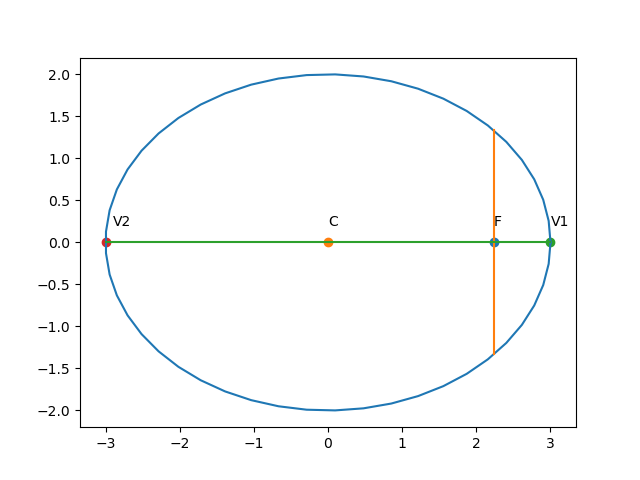
\includegraphics[width=\columnwidth]{figs/Figure_1.png}
    \caption{Figure 1}
    \label{fig:}
\end{figure}

\end{document}



